\section{Tarea}


\begin{itemize}
    \item \textbf{URL GitHub de Tarea del Ajedrez:} \url{https://github.com/rescobedoq/pw2/tree/main/labs/lab04/Tarea-del-Ajedrez}
    \item En esta tarea usted pondrá en práctica sus conocimientos de programación en Python para dibujar un tablero de Ajedrez.
    \item La parte gráfica ya está programada, usted sólo tendrá que concentrarse en las estructuras de datos subyacentes.
    \item Con el código proporcionado usted dispondrá de varios objetos de tipo Picture para poder realizar su tarea:
\end{itemize}
\subsection{Una vez instalado python y creado un virtual environment para la resolucion de este laboratorio 
	nos fijamos en el repositorio de github compartido por el profesor y nos fijamos que una de 
	las dependencias es el modulo de python pyGame, lo instalamos con pip y descargamos el codigo fuente.}

\begin{lstlisting}[style=mybash]
	pip3 install pygame
	curl -LJO https://github.com/rescobedoq/pw2/blob/main/labs/lab04/Tarea-del-Ajedrez/chessPictures.py
	curl -LJO https://github.com/rescobedoq/pw2/blob/main/labs/lab04/Tarea-del-Ajedrez/colors.py
	curl -LJO https://github.com/rescobedoq/pw2/blob/main/labs/lab04/Tarea-del-Ajedrez/interpreter.py
	curl -LJO https://github.com/rescobedoq/pw2/blob/main/labs/lab04/Tarea-del-Ajedrez/picture.py
	curl -LJO https://github.com/rescobedoq/pw2/blob/main/labs/lab04/Tarea-del-Ajedrez/pieces.py
\end{lstlisting}

\begin{itemize}
    \item Estos objetos estarán disponibles importando la biblioteca: \texttt{chessPictures} y estarán internamente representados con arreglos de strings que podrá revisar en el archivo \texttt{pieces.py}.
    \item La clase \texttt{Picture} tiene un sólo atributo: el arreglo de strings \texttt{img}, el cual contendrá la representación en caracteres de la figura que se desea dibujar.
    \item La clase \texttt{Picture} ya cuenta con una función implementada, no debe modificarla, pero sí puede usarla para implementar sus otras funciones:
    \item La clase Picture contará además con varios métodos que usted deberá implementar
    \item \begin{itemize}
		\item \texttt{verticalMirror}: Devuelve el espejo vertical de la imagen
		\item \texttt{horizontalMirror}: Devuelve el espejo horizontal de la imagen
		\item \texttt{negative}: Devuelve un negativo de la imagen
		\item \texttt{join}: Devuelve una nueva figura poniendo la figura del argumento al lado derecho de la figura actual
		\item \texttt{up}: Devuelve una nueva figura poniendo la figura recibida como argumento, encima de la figura actual
		\item \texttt{under}: Devuelve una nueva figura poniendo la figura recibida como argumento, sobre la figura actual
		\item \texttt{horizontalRepeat}: Devuelve una nueva figura repitiendo la figura actual al costado la cantidad de veces que indique el valor de \texttt{n}
		\item \texttt{verticalRepeat}: Devuelve una nueva figura repitiendo la figura actual debajo, la cantidad de veces que indique el valor de \texttt{n}
	\end{itemize}	
\end{itemize}

	El primer paso de la tarea es entonces implementar estos metodos en python para usarlos en la tarea
	\begin{lstlisting}
		RUN apt-get install -y mariadb-server
	\end{lstlisting}

	\subsection{Cree un usuario pweb2 con contraseña: 12345678. \newline
	Otorgue permisos al usuario para acceder a la aplicación web. (Read/Write) \newline}

	Esta operacion se realizo a travez del terminal del container una vez creado la imagen y corriendo,
	En resumen el dockerfile que utilizo para crear la imagen se ve tal que asi:

	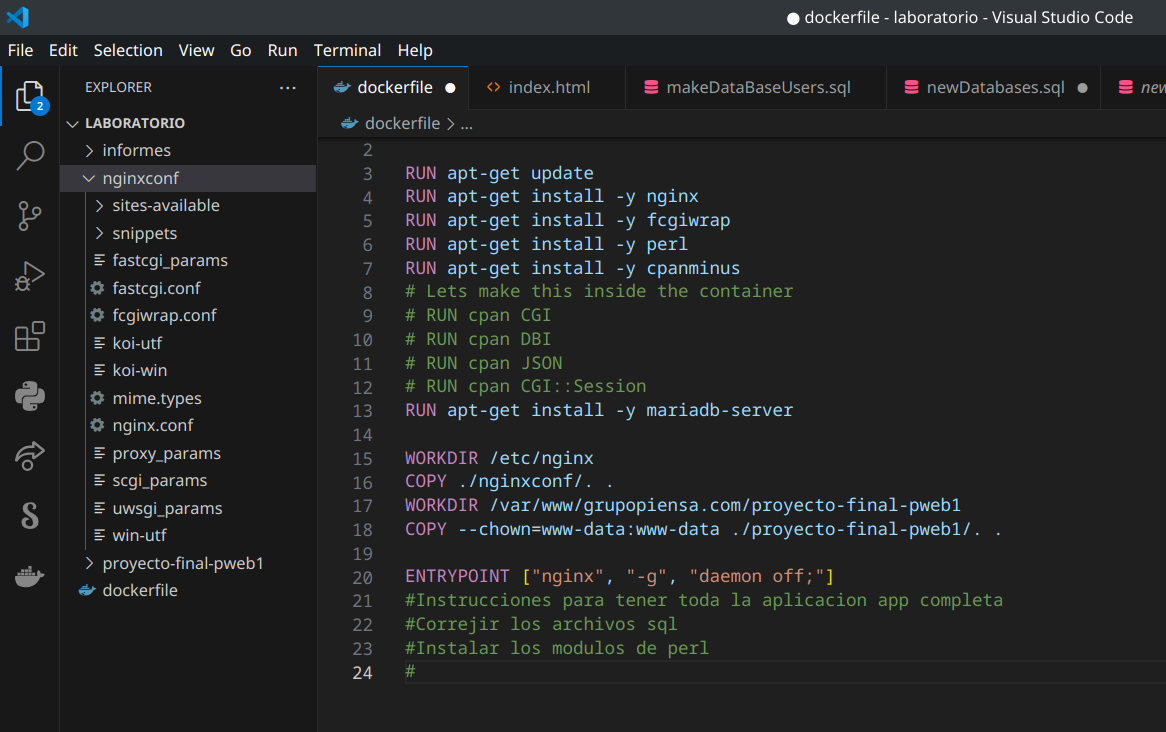
\includegraphics[scale=0.4]{./img/lab1_1.png}
	
	Una vez adentro del terminal del contenedor puedo comenzar los procesos de MariaDB asi como el servicio de fcgiwrap
	el cual me permite ejecutar cgi en servidores estaticos administrados por nginx.\newline \newline

	\begin{lstlisting}[style=mybash]
		docker run -dp 8000:80 nginxserver
		docker exec -it mystifying_ellis /bin/bash
		root@1a30749290f4:/var/www/grupopiensa.com/proyecto-final-pweb1# /etc/init.d/mariadb start
		 * Starting MariaDB database server mariadbd                                                                                                                                         [ OK ] 
		root@1a30749290f4:/var/www/grupopiensa.com/proyecto-final-pweb1# /etc/init.d/fcgiwrap start
		 * Starting FastCGI wrapper fcgiwrap                                                                                                                                                 [ OK ] 
		root@1a30749290f4:/var/www/grupopiensa.com/proyecto-final-pweb1# mysql
		Welcome to the MariaDB monitor.  Commands end with ; or \g.
		Your MariaDB connection id is 33
		Server version: 10.6.16-MariaDB-0ubuntu0.22.04.1 Ubuntu 22.04

		Copyright (c) 2000, 2018, Oracle, MariaDB Corporation Ab and others.

		Type 'help;' or '\h' for help. Type '\c' to clear the current input statement.

		MariaDB [(none)]> create database pweb1
		    -> ;
		Query OK, 1 row affected (0.001 sec)		
		MariaDB [(none)]> GRANT ALL PRIVILEGES ON pweb1.* TO 'alumno'@'%' IDENTIFIED BY 'pweb1';
		Query OK, 0 rows affected (0.015 sec)

		MariaDB [(none)]> exit
		Bye

	\end{lstlisting}

	\subsection{Finalmente implemente el trabajo final del curso de pw1 en ese contenedor. \newline
	Elabore un informe paso a paso para donde explique funcionalmente el proyecto demostrando  que se trata de un contenedor docker.\newline
	Adjunte la URL de un video donde muestre que se trata de un contenedor Docker. \newline}

	Entonces para probar mi contenedor de docker que este correctamente sirviendo los servidores de nginx voy a entrar al buscador de firefox 
	y buscar la pagina web grupopiensa, el cual esta mapeado al localhost 127.0.0.1 en el puerto 8000, el cual tiene un port forwarding
	al puerto 80 del contenedor

	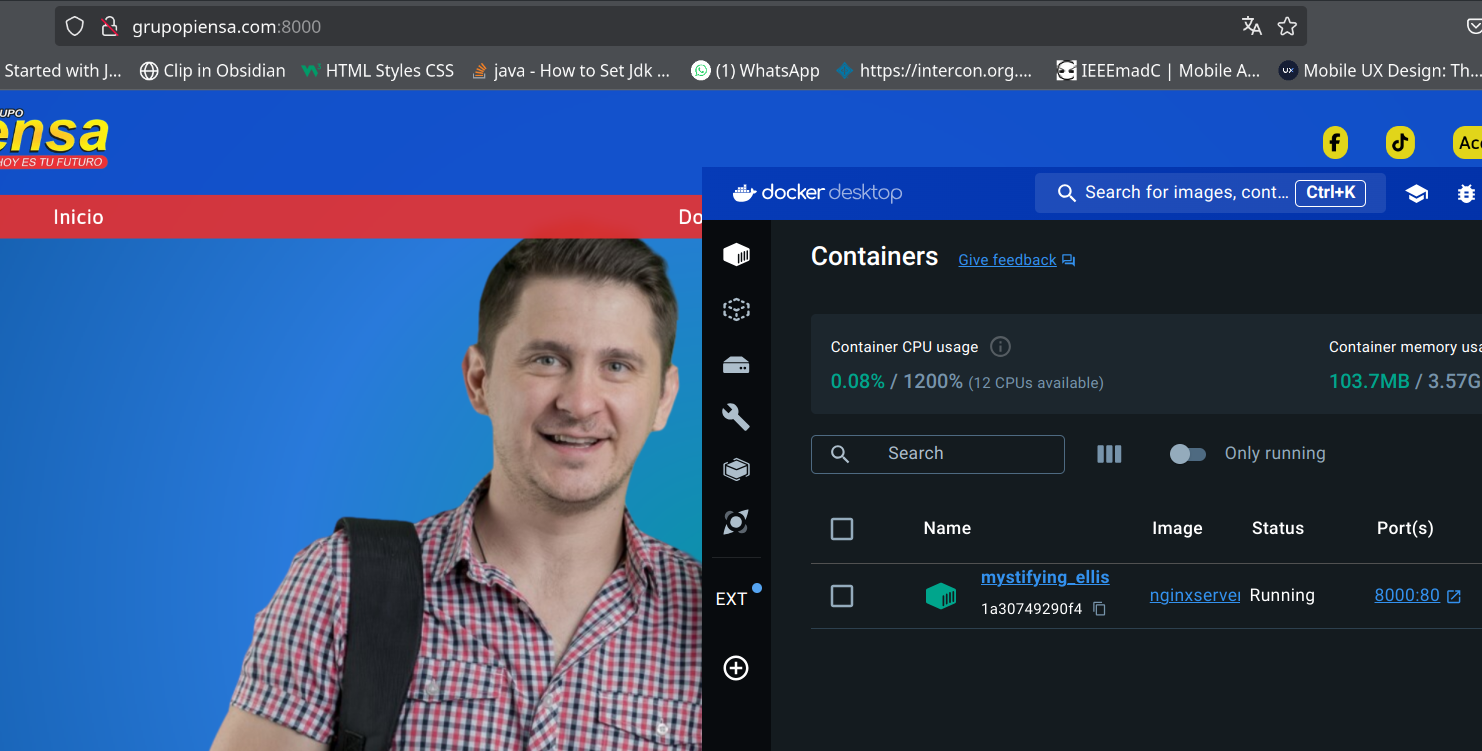
\includegraphics[scale = 0.3]{./img/lab1_2.png}
	\newline
	Aqui dejo el enlace al video de YT en el que se muestra la veracidad del uso de Docker para hostear paginas web: https://youtu.be/ERklT6IMV7E

\pagebreak